
\section{PC Blokken}

\subsection{Action (Kristian T.)}

\begin{figure}[h]
\centering
\includegraphics[scale=1,clip=true, trim=389 282 302 204.7]{Systemarkitektur/diagrammer/PC_KlasseDiagram} %L B R T - HUSKE DET
\caption{Action klassen}
\end{figure}

%setCommand (1)
\begin{table}[h] 
\begin{tabularx}{\textwidth}{p{0.6 cm} l X} %\hline
\multicolumn{3}{l}{\textbf{setCommand}}\\
& Operation: & %Skriv tekst herunder
\texttt{bool setCommand( int commandNo )}
\\ & Parametre: & %Skriv tekst herunder
Modtager nummeret på den kommando der skal eksekveres.

1 = Tænd

2 = Sluk

3 = Dim 5\%

4 = Dim 15\%

\ldots 

12 = Dim 95\%

\\ & Returværdi: & %Skriv tekst herunder
Returnerer \texttt{TRUE}, hvis input var gyldigt og \texttt{FALSE} hvis ikke.
\\ & Beskrivelse: & %Skriv tekst herunder
Set-metode til at vælge hvilken kommando, den givne aktion skal indeholde. Metoden ændrer udelukkende på variablerne \texttt{commandNo}.
\\ \end{tabularx}
\end{table}

%setUnit
\begin{table}[h] 
\begin{tabularx}{\textwidth}{p{0.6 cm} l X} %\hline
\multicolumn{3}{l}{\textbf{setUnit}}\\
& Operation: & %Skriv tekst herunder
\texttt{bool setUnit( int unitNo )} 
\\ & Parametre: & %Skriv tekst herunder
Modtager hvilken enhed aktionen skal manipulere.

1 = Lampe 1

2 = Lampe 2

3 = TV

4 = Radio

Alle andre værdier er ugyldige. 
\\ & Returværdi: & %Skriv tekst herunder
Returnerer \texttt{TRUE}, hvis input var gyldigt og \texttt{FALSE} hvis ikke.
\\ & Beskrivelse: & %Skriv tekst herunder
Set-metode til at vælge hvilken enhed, den givne aktion skal manipulere. Metoden ændrer udelukkende på variablerne \texttt{houseCode} og \texttt{unitCode}. \texttt{houseCode} skal iøvrigt sættes i forhold til den enhed, som vælges. Lampe 1 og Lampe 2 er under huskode 1, TV og Radio er under hhv. 2 og 3.
\\ \end{tabularx}
\end{table}

%setTime
\begin{table}[h] 
\begin{tabularx}{\textwidth}{p{0.6 cm} l X} %\hline
\multicolumn{3}{l}{\textbf{setTime}}\\
& Operation: & %Skriv tekst herunder
\texttt{bool setTime( int time ) }
\\ & Parametre: & %Skriv tekst herunder
Modtager tidspunktet for hvornår en aktion skal udføres i minutter fra kl \texttt{00:00}. Dvs hvis en aktion skal starte kl \texttt{15:30} skal værdien $15 \times 60 + 30 = 930$ indsættes.
\\ & Returværdi: & %Skriv tekst herunder
Returnerer \texttt{TRUE}, hvis input var gyldigt og \texttt{FALSE} hvis ikke.
\\ & Beskrivelse: & %Skriv tekst herunder
Set-metode til at vælge hvilket tidspunkt, den givne aktion skal udføres. Metoden ændrer udelukkende på variablen \texttt{minutes}.
\\ \end{tabularx}
\end{table}

%operator<<
\begin{table}[h] 
\begin{tabularx}{\textwidth}{p{0.6 cm} l X} %\hline
\multicolumn{3}{l}{\textbf{operator{<}{<}}}\\
& Operation: & %Skriv tekst herunder
\texttt{ostream \& operator{<}{<}( ostream \& theStream, Action \& theAction ) }
\\ & Parametre: & %Skriv tekst herunder
Modtager et \texttt{ostream} objekt, som der skal streames til samt en reference til et objekt af klassen \texttt{Action}, som skal udskrives.
\\ & Returværdi: & %Skriv tekst herunder
Returnerer en reference til det \texttt{ostream} objekt, som metoden blev kaldt med (tillader cascading).
\\ & Beskrivelse: & %Skriv tekst herunder
Udskriver en linie med tidspunkt i formattet \texttt{HH:MM}, enhedsnavn og kommando beskrevet i tekstform, afsluttet med et linieskift.
\\ \end{tabularx}
\end{table}

%Explicit constructor
\begin{table}[h] 
\begin{tabularx}{\textwidth}{p{0.6 cm} l X} %\hline
\multicolumn{3}{l}{\textbf{Explicit constructor}}\\
& Operation: & %Skriv tekst herunder
\texttt{Action( int time, int unit,  int commandNo ) }
\\ & Parametre: & %Skriv tekst herunder
Modtager parametre for hhv. tid, enhed og kommandonummer.
\\ & Beskrivelse: & %Skriv tekst herunder
Initierer attributter i objektet, skal sætte attributterne til passende default-værdier, hvis ingen værdier gives.
\\ \end{tabularx}
\end{table}

\begin{table}[h]
\centering
\begin{tabularx}{13 cm}{|l |X|} \hline
Attribut & Beskrivelse \\ \hline
\texttt{int seconds} & Tiden fra kl \texttt{00:00} til tiden for at den pågældende aktion skal udføres i sekunder. \\ \hline
\texttt{int houseCode} & Huskoden for den enhed, som aktionen skal manipulere. \\ \hline
\texttt{int unitCode} & Enhedskoden for den enhed, som aktionen skal manipulere. \\ \hline
\texttt{int commandNo} & Nummeret på den kommando, som skal eksekveres. \\ \hline
\end{tabularx}
\end{table}

\clearpage

\subsection{PC Controller}

\begin{figure}[h]
\centering
\includegraphics[scale=1,clip=true, trim=267 444 473 60]{Systemarkitektur/diagrammer/PC_KlasseDiagram} %L B R T - HUSKE DET
\end{figure}

PC controlleren virker som et main program, og holder styr på følgende:

\begin{itemize}
\item Kodelås
\item Data til UART klassen
\item Led mellem Scenario og UI klassen
\end{itemize}

\subsection{Scenario (Kristian S.)}

\begin{figure}[h]
\centering
\includegraphics[scale=1,clip=true, trim=149 320 541 224]{../Projektdokumentation/Systemarkitektur/diagrammer/PC_KlasseDiagram.pdf} %L B R T - HUSKE DET
\end{figure}

\begin{table}[h]
\begin{tabularx}{\textwidth}{p{0.6 cm} l X} %\hline
\multicolumn{3}{l}{\textbf{Constructor}}\\
& Operation: & 
\texttt{void Scenario()}  
\\ & Parametre: & 
-
\\ & Returværdi: & 
-
\\ & Beskrivelse: & 
constructoren opretter et array med 20 objekter af klassen action i.
\\ \end{tabularx}
\end{table}

\begin{table}[h]
\begin{tabularx}{\textwidth}{p{0.6 cm} l X} %\hline
\multicolumn{3}{l}{\textbf{getAction}}\\
& Operation: & 
\texttt{Action \& getAction(int actionNo)}  
\\ & Parametre: & 
actionNo - ID'et på den action er der skal bruges
\\ & Returværdi: & 
Action \& - Reference til den valgte action.
\\ & Beskrivelse: & 
Methoden finder den valgte Action ud fra parameteren \texttt{actionNo}, og returnere en reference til den action.
\\ \end{tabularx}
\end{table}
\clearpage

\begin{table}[h]
\begin{tabularx}{\textwidth}{p{0.6 cm} l X} %\hline
\multicolumn{3}{l}{\textbf{sortActions}}\\
& Operation: & 
\texttt{Action[] \& sortActions( Action[] )}  
\\ & Parametre: & 
Modtager en pointer til et array af \texttt{Action} objekter.
\\ & Returværdi: & 
Returnerer en reference til det sorterede array af \texttt{Action} objekter.
\\ & Beskrivelse: & 
Sorterer et array af \texttt{Action} objekter efter udførelsestidspunkt. Den der skal udføres først lægges i starten af arrayet. Alt skal være relativt til det nuværende tidspunkt.
\\ \end{tabularx}
\end{table}

%operator<<
\begin{table}[h]
\begin{tabularx}{\textwidth}{p{0.6 cm} l X} %\hline
\multicolumn{3}{l}{\textbf{operator{<}{<}}}\\
& Operation: & 
\texttt{ostream \& operator{<}{<}( ostream \& theStream, Scenario \& theScen )}  
\\ & Parametre: & 
Modtager det \texttt{ostream} objekt, som der skal streames til samt hvilket \texttt{Scenario} objekt, der skal streames.
\\ & Returværdi: & 
Returnerer en reference til det \texttt{ostream} objekt, der modtages som parameter. (tillader cascading).
\\ & Beskrivelse: & 
Skal udskrive ''Aktionsnummer  Tidspunkt  Enhed  Kommando'' som titler med et bestemt mellemrum på én linie og herefter udskrive nummeret på den første aktion, den første aktion på den næste linie. Herefter udskrives nummeret på den anden aktion samt den anden aktion på den næste linie osv. Se evt. Tabel \ref{tbl:kommando} på side \pageref{tbl:kommando} i kravspecifikationen.
\\ \end{tabularx}
\end{table}

%\clearpage

\subsection{UART (Kasper)}

\begin{figure}[h]
\centering
\includegraphics[scale=1,clip=true, trim=448 440 225 50]{Systemarkitektur/diagrammer/PC_KlasseDiagram} %L B R T - HUSKE DET
\end{figure}

UART'en laves med udgangspunkt i funktionerne fra et open-source UART projekt. \cite{lib:UART}

\begin{table}[h]
\begin{tabularx}{\textwidth}{p{0.6 cm} l X} %\hline
\multicolumn{3}{l}{\textbf{Connect}}\\
& Operation: & 
\texttt{Void Connect()}
\\ & Parametre: & 
 - 
\\ & Returværdi: & 
-
\\ & Beskrivelse: & 
Connect methoden bruges til at finde en gyldig USB port hvor i der er indsat et RS-232 stik som bruges til seriel kommunikation. metoden løber igennem alle gyldige COM-porte på PC'en indtil en port, med RS-232 stik i, findes.
\\ \end{tabularx}
\end{table}
\clearpage

\begin{table}[h]
\begin{tabularx}{\textwidth}{p{0.6 cm} l X} %\hline
\multicolumn{3}{l}{\textbf{getLockStatus}}\\
& Operation: & 
\texttt{bool getLockStatus( void)}
\\ & Parametre: & 
 - 
\\ & Returværdi: & 
bool: returnere \texttt{true} / \texttt{false} afhængeligt af kodelåsens status.
\\ & Beskrivelse: & 
Sender ASCII værdien for et \texttt{L} over til microcontrolleren for at få kodelåsens status. Funktionen venter på at få et svar tilbage fra microcontrolleren, hvilket er ASCII værdien for et \texttt{U} eller et \texttt{L}.
Hvis UART'en får et \texttt{L} returneres \texttt{True}.
Hvis UART'en får et \texttt{U} returneres \texttt{False}.
\\ \end{tabularx}
\end{table}

\begin{table}[h]
\begin{tabularx}{\textwidth}{p{0.6 cm} l X} %\hline
\multicolumn{3}{l}{\textbf{stopAll}}\\
& Operation: & 
\texttt{void stopAll(void)}
\\ & Parametre: & 
 - 
\\ & Returværdi: & 
-
\\ & Beskrivelse: & 
Funktionen bruges til at slukke for alle enheder tilsluttet systemet. ASCII værdien for et \texttt{S} sendes for til  microcontrolleren. Se evt. Protokol for UART side \pageref{prot_UART}.
\\ \end{tabularx}
\end{table}

\begin{table}[h]
\begin{tabularx}{\textwidth}{p{0.6 cm} l X} %\hline
\multicolumn{3}{l}{\textbf{sendScen}}\\
& Operation: & 
\texttt{void sendScen(Scenario \& Scenario)}
\\ & Parametre: & 
 Scenario \& Scenario: reference til scenariet.
\\ & Returværdi: & 
-
\\ & Beskrivelse: & 
UARTen transmittere data over serial kommunikation. Rækkefølgen på data der bliver sendt er følgende:
Unit (1 char) \- CMD(1char) \- Time (3 char).
datarækken bliver sendt 20 gange for at få alle kommandoer i scenariet overført til microcontroller. 		

NOTE: Tiden omreges iforhold til nuværende tid på systemet i computeren.
f.eks. hvis klokken er 15.00 på computeren og første aktion sker kl 16.30 bliver tiden sat som 90.

\\ \end{tabularx}
\end{table}

\clearpage

\subsection{UI (Kasper)}
 
\begin{figure}[h]
\centering
\includegraphics[scale=1,clip=true, trim=38 433 625 50]{../Projektdokumentation/Systemarkitektur/diagrammer/PC_KlasseDiagram} %L B R T - HUSKE DET
\end{figure}

\begin{table}[h]
\begin{tabularx}{\textwidth}{p{0.6 cm} l X} %\hline
\multicolumn{3}{l}{\textbf{drawMainMenu}}\\
& Operation: & 
\texttt{int drawMainMenu( void )} 
\\ & Parametre: & 
 -
\\ & Returværdi: & 
int : Den returnerede integer er hvilken menu der er valgt.
\\ & Beskrivelse: & 
Metoden udskriver en menu over de forskellige undermenuer på skærmen og giver brugeren muligheden for at vælge at gå ind i en af undermenuerne (opret nyt scenarie(1), kør eksisterende scenarie(2), stop scenarie(3)). Der fortages et tjek på det indtastede af brugeren, som skal valideres. validationen tjekker at det indtastede er enten 1,2 eller 3 som er de gyldige menu'er. hvis det indtastede er ugyldigt får brugeren en besked om ugyldigt input og får lov at forsøge igen. Dette sker indtil brugeren indtaster noget gyldigt.
\\
\end{tabularx}
\end{table}

\begin{table}[h]
\begin{tabularx}{\textwidth}{p{0.6 cm} l X} %\hline
\multicolumn{3}{l}{\textbf{drawScenario}}\\
& Operation: & 
\texttt{int drawScenario( Scenario \& currentScen )} 
\\ & Parametre: & 
Scenario \& currentScen : reference til klassen Scenario
\\ & Returværdi: & 
int : Den returnerede værdi er den valgte action i Scenariet
\\ & Beskrivelse: & 
Metoden udskriver en liste over de 20 aktioner der er i scenariet med at bruge ostream operatoeren der er lavet i klassen \texttt{Scenarie}. Brugeren kan derefter vælge hvilken af de 20 aktioner der skal redigeres ved at indtaste nummeret på aktionen. Når brugeren har indtastet noget, valideres dette. Hvis inputtet er den af de gyldige værdier (0-19), returneres ID'et/den gyldige værdi. Hvis inputtet er ugyldigt får brugeren en besked om ugyldigt input og får lov at forsøge igen. Dette sker indtil brugeren indtaster noget gyldigt.
\\
\end{tabularx}
\end{table}

\begin{table}[h]
\begin{tabularx}{\textwidth}{p{0.6 cm} l X} %\hline
\multicolumn{3}{l}{\textbf{drawAskUnits}}\\
& Operation: & 
\texttt{int drawAskUnits( void )} 
\\ & Parametre: & 
 -
\\ & Returværdi: & 
int : Den returnerede integer er hvilken unit der valgt
\\ & Beskrivelse: & 
Metoden udskriver en liste over units. hvor unitsne er: Lampe1, Lampe2, TV og Radio.
brugeren kan derefter vælge hvilke af de 4 units der skal bruges, ved at indtaste nummeret på unit'en.
Når brugeren har indtastet noget, valideres dette. Hvis inputtet er en af de gyldige værdier (1-4) returneres unit ID'en/den gyldige værdi. Hvis inputtet er ugyldigt får brugeren en besked om ugyldigt input og får lov at forsøge igen. Dette sker indtil brugeren indtaster noget gyldigt.
\\
\end{tabularx}
\end{table}

\begin{table}[h]
\begin{tabularx}{\textwidth}{p{0.6 cm} l X} %\hline
\multicolumn{3}{l}{\textbf{drawAskCommando}}\\
& Operation: & 
\texttt{int drawAskCommand( void )} 
\\ & Parametre: & 
 -
\\ & Returværdi: & 
int : Den returnerede integer er hvilken kommando
\\ & Beskrivelse: & 
Metoden udskriver en liste over kommandoer. Brugeren kan derefter vælge hvilken kommando der skal bruges, og ID'en på denne kommando returneres. 
\\
\end{tabularx}
\end{table}

\begin{table}[h]
\begin{tabularx}{\textwidth}{p{0.6 cm} l X} %\hline
\multicolumn{3}{l}{\textbf{drawAskTime}}\\
& Operation: & 
\texttt{int drawAskTime( void )} 
\\ & Parametre: & 
 -
\\ & Returværdi: & 
int : tiden i minutter indtastet af brugeren siden kl 00.00
\\ & Beskrivelse: & 
Metoden beder brugeren om at indtaste den ønskede time-tal, hvor en ønsket kommando skal udføres. Brugeren kan derefter indtaste det ønskede time-tal. 
Metoden beder nu brugeren om at indtaste det ønskede minut-tal i den ønskede time. Brugeren kan nu indtaste det ønskede minut-tal. Metoden validere nu time- og minut-tallene. hvis time-talet er indenfor det gyldige område (0-23) og minut-talet er indenfor dens gyldige område (0-59), udregnes tiden i minutter siden kl 00.00 og returneres. Hvis enten minut- eller time-tal er udenfor det gyldige område, køres metoden fra starten af, og dette sker indtil den gyldig tid indtastes.
\\
\end{tabularx}
\end{table}

\begin{table}[h]
\begin{tabularx}{\textwidth}{p{0.6 cm} l X} %\hline
\multicolumn{3}{l}{\textbf{drawScenList}}\\
& Operation: & 
\texttt{int drawScenList( void )} 
\\ & Parametre: & 
 -
\\ & Returværdi: & 
int : ID'et på det valgte scenarie
\\ & Beskrivelse: &
Brugeren bliver præsenteret for 3 forudstillede scenarier, med beskrivelser af hvad de gør. Brugeren vælger en af de 3 forudinstillet scenarier, ved at indtaste nummeret på det ønskede scenarie. Det indtastede valideres. Hvis det indtastede er indenfor området 1-3, returneres det indtastede, ellers bliver brugeren bedt om at prøve igen, indtil noget gyldigt er indtastet.
\end{tabularx}
\end{table}

\clearpage

\begin{table}[h]
	\begin{tabularx}{\textwidth}{p{0.6 cm} l X} %\hline
	\multicolumn{3}{l}{\textbf{drawStopPromt}}\\
	& Operation: & 
	\texttt{bool drawStopPromt( void )} 
	\\ & Parametre: & 
	 -
	\\ & Returværdi: & 
	bool: returnere \texttt{true} for valgt 'ja' og \texttt{false} for valgt nej
	\\ & Beskrivelse: & 
	Brugeren bliver præsenteret med muligheden om brugeren er sikker på at scenariet skal afsluttes. Hvis brugeren trykker på \texttt{Y / y} tasten returneres dette som et \texttt{true}, altså et 'ja'. hvis alt andet end \texttt{Y / y} trykkes returneres \texttt{false}, svarende til et 'nej'.
\end{tabularx}
\end{table}

\clearpage
